\documentclass[
  ngerman
  ,12pt
  ,pdftex
]{report}

\usepackage{mitschrieb}


\hyphenation{Differential-gleichung}
\hyphenation{Über-tragungs-ope-ra-tors}
\hyphenation{E/A-Dif-fe-ren-ti-al-glei-chung}

\begin{document}

\begin{titlepage}
  \begin{center}
      {\Huge \textbf{Programmentwurf: Wer ist der Spion?}}\\[1.5cm]
      {\Large Lorenz Scherrer}\\[1cm]
      {\Huge Advanced Software}\\[7cm]
      {\large Matrikelnummer: \textbf{8809469}}\\[0.5cm]
      %{\large Matrikelnummer: \textbf{6130555}}\\[0.5cm]
      {\large Kurs: TINF21B3}\\[0.5cm]
      {\large Abgabedatum 16.12.2022}
      \vfill
  \end{center}
\end{titlepage}
\newpage
\tableofcontents
\newpage

% INPUTS
\chapter{Beschreibung der Funktionalität: Wer ist der Spion?}
Die entwickelte App ist eine digitale Umsetzung des beliebten Gesellschaftsspiels "Wer ist der Spion?". Ziel der App ist es, den Spaß und die Spannung des Spiels auf Mobilgeräte zu bringen und es den Benutzern zu ermöglichen, jederzeit und überall zu spielen. Die Hauptfunktionen der App umfassen:

\begin{itemize}
    \item \textbf{Spielrunden erstellen:} Benutzer können neue Spielrunden erstellen und Mitspieler einladen, entweder aus ihrer Kontaktliste oder durch Generierung eines Einladungslinks.
    \item \textbf{Rollen zuweisen:} Die App weist automatisch jedem Spieler eine Rolle zu, entweder als normaler Spieler mit Kenntnis des geheimen Themas oder als Spion, der das Thema nicht kennt.
    \item \textbf{Fragen stellen und Antworten geben:} Die Spieler können sich gegenseitig Fragen stellen, um Hinweise auf das geheime Thema zu erhalten, während der Spion versucht, das Thema zu erraten, ohne entdeckt zu werden.
    \item \textbf{Punkte vergeben und Spielstatistiken anzeigen:} Die App verfolgt die Spielrunden und Punkteverteilung, um den Spielfortschritt zu verfolgen, und zeigt den Spielern ihre Statistiken an.
\end{itemize}

\section{Beschreibung des Kundennutzens:}

Die App bietet den Benutzern eine unterhaltsame und interaktive Möglichkeit, das Spiel "Wer ist der Spion?" zu spielen, ohne physische Karten oder Zubehör zu benötigen. Der Kundennutzen umfasst:

\begin{itemize}
    \item \textbf{Flexibilität:} Spieler können das Spiel jederzeit und überall spielen, indem sie einfach ihre Mobilgeräte verwenden.
    \item \textbf{Soziale Interaktion:} Das Spiel fördert die soziale Interaktion zwischen den Spielern, da sie sich gegenseitig Fragen stellen und versuchen, den Spion zu entlarven.
    \item \textbf{Spaß und Spannung:} Die App bietet den Spielern die Möglichkeit, den Nervenkitzel des Spiels zu erleben, während sie versuchen, das geheime Thema zu erraten oder ihre wahre Identität als Spion zu verbergen.
\end{itemize}



\subsection{Verwendete Technologie}
Die Anwendung wird in Kotlin entwickelt, einer modernen und leistungsstarken Programmiersprache, die sich besonders gut für die Entwicklung von Android-Apps eignet. Weitere Technologien und Frameworks umfassen:
\begin{itemize}
    \item \textbf{Back-End:} Kotlin 
    \item \textbf{Front-End-Framework:} Kotlin-Ktor Client
    \item \textbf{Entwicklungsumgebung:}  IDE oder Code-Editor
\end{itemize}


\subsection{Ausführbare Datei}

Man kann das Projekt als Jar kompilieren und ausführen lassen. Unter diesem \href{https://github.com/lorenz1702/Spy-Game/commit/ea4fd2fed71a7a43e10448dd173c79ca53789201}{Commit-Hash} unter build/libs/SpyGame.jar

\newpage
\chapter{Clean Architecture}
Die Clean Architecture ist ein Architekturmuster, das darauf abzielt, Softwareprojekte gut strukturiert, wartbar und testbar zu gestalten. Ein zentrales Thema bei der Entwicklung von Software ist die Wahl zwischen der Verwendung von Libraries und Frameworks. In diesem Kontext wird argumentiert, dass es oft vorteilhafter ist, auf Libraries zurückzugreifen anstatt auf Frameworks zu setzen.\\

\section{Kriterien für nachhaltige Architektur}
\begin{itemize}
\item besitzt einen technologieunabhängigen Kern: der Domain und Applikation ist nur aus Kotlin Code ohne Bibliotheken.
\item behandelt jede Abhängigkeit als temporäre Lösung
\item Unterscheidet zwischen zentralem (\textit{langlebigem}) und peripherem (\textit{kurzlebigem}) Sourcecode
\item \textbf{Metapher:} Die Zwiebel - alle Änderungen sollen den Kern nicht verändern
\end{itemize}

\textbf{Peripherie}: Hier werden die kurzlebigen Bibliotheken an den Kern angebunden. Abhängigkeiten gehen nur vom peripheren Code in den Kern, nie umgekehrt.

\section{Dependency Inversion}
\label{sec:DI}
:Interfaces verwenden damit der Kern Code nicht verändert werden muss. Es kann auch anders gelöst werden die Programmiersprache braucht keine interfaces.
Die Kern-Klasse muss die andere nicht kennen. Schalter(\textbf{Kern}), Schalterbar(\textbf{Plugin}), Lampe/Ventilator(\textbf{Bibliotheken})\\
So in der Theorie.

Um die Dependency Inversion zu erreichen, werden wir eine Abstraktion einführen, die es uns ermöglicht, WordRepository von der konkreten GameLogic-Klasse zu entkoppeln. Wir erstellen eine Schnittstelle für die GameLogic-Klasse und lassen ImplWordRepsoitory stattdessen von dieser Schnittstelle abhängen.

\lstinputlisting[caption={Example for Dependency Inversion}, label={lst:example1}, language=Kotlin]{images/DependencyInversion.kt}

Der Applikation Code ruft Code aus der Adapter Layer auf ohne es zu merken\href{https://github.com/lorenz1702/Spy-Game/commit/280bfad83aeff3a2e16b78514f29b766b8f8259f}{Commit-Hash}. 

Die GameLogic-Klasse kennt also nicht die konkreten Implementierungen der Methoden in den Repositories. Stattdessen verwendet sie die definierten Methoden des Interfaces. Dies ermöglicht eine hohe Flexibilität und Austauschbarkeit der Implementierungen. Zum Beispiel kann die GameLogic-Klasse problemlos mit einer anderen Implementierung des UserRepository arbeiten, solange diese die gleichen Methoden des UserRepository-Interfaces implementiert.
    
Durch die Verwendung von abstrakten Interfaces und die Abhängigkeit von ihnen anstelle von konkreten Implementierungen wird das Prinzip der Dependency Inversion erreicht, was eine lockerere Kopplung und eine bessere Testbarkeit der GameLogic-Klasse ermöglicht.

Hier sieht man noch die Dependency Inversion bildlich dargestellt \ref{fig:14}.

\begin{figure}[h]
    \centering
    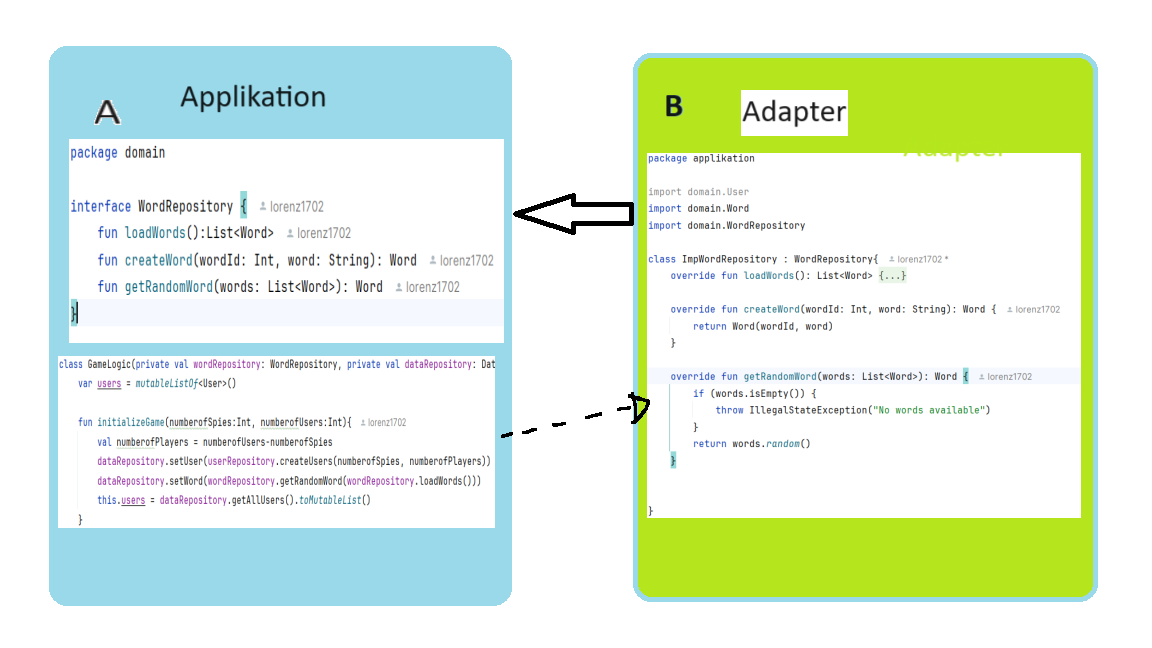
\includegraphics[width=17cm]{images/Denpendancy Inversion.png}
    \caption{Dependency Inversion}%
    \label{fig:14}
\end{figure}

\section{Struktur der Clean Architecture}

\subsection{Domain Code}

In diesem Bereich wird die Benutzer-Entität definiert. 

\subsection{Applikationscode}

Hier werden die Anwendungsfälle (Use Cases) implementiert, die die Kernfunktionalität der Anwendung umsetzen.


\subsection{Plugin}

Adapter dienen als Vermittler zwischen der Daten und der inneren Schicht der Anwendung. Sie übermitteln Daten und führen Aufrufe der inneren Schicht aus. Des Weiteren konvertieren sie Datentypen.



\subsection{Adapter}

Die Adapter-Schicht, die den Ktor-Server implementiert, zeichnet sich durch ihre hohe Austauschbarkeit und Flexibilität aus. Diese Schicht fungiert als Schnittstelle zwischen dem Anwendungskern und dem Ktor-Framework, das für die Verarbeitung von HTTP-Anfragen und -Antworten verantwortlich ist.

Durch die Verwendung des Adaptermusters kann die Implementierung des Ktor-Servers leicht ausgetauscht werden, ohne dass dies Auswirkungen auf den Rest der Anwendung hat. Dies ermöglicht es, verschiedene Implementierungen des Servers zu verwenden, je nach den spezifischen Anforderungen oder Präferenzen des Projekts.

Die Austauschbarkeit der Adapter-Schicht bietet auch die Möglichkeit, verschiedene Technologien oder Frameworks zu evaluieren und zu testen, ohne dass dies größere Änderungen am Anwendungskern erfordert. Dies fördert die Flexibilität und Erweiterbarkeit der Anwendung und erleichtert die Wartung und Weiterentwicklung im Laufe der Zeit.\\

\textbf{Funktionsweise von Serveraufrufen}

Die Funktionalität der Serveraufrufe soll eine Schnittstelle bereitstellen, um Daten zwischen dem Server und der Anwendungslogik auszutauschen.



\subsection{Framework vs. Library}
\textbf{Problem}:
Das Problem von Abhängigkeiten ist, dass sie sich immer ändern, je nach den Frameworks, mit denen man arbeitet. Die verwendeten Frameworks ändern sich alle 5-10 Jahre. Wenn man nicht alle 5 Jahre alles neu machen möchte, muss man die Abhängigkeiten auflösen.

\textbf{Lösung}:
Entscheidungen am besten möglichst spät treffen. \textbf{Minimalziel}:
Entscheidungen müssen revidierbar sein können $\Longrightarrow$ mit möglichst geringen negativen Folgen.

Im Gegensatz dazu bieten Libraries nur spezifische Funktionen oder Werkzeuge, ohne eine vorgegebene Struktur aufzuerlegen. Dies ermöglicht es Entwicklern, die Bibliotheken selektiv und flexibel einzusetzen, je nach den Anforderungen ihres Projekts. Sie bleiben weniger anfällig für Änderungen in der Technologielandschaft, da sie weniger in die Infrastruktur des Projekts eingebettet sind.\\

Durch die Verwendung von Libraries statt Frameworks wird die Abhängigkeit umgekehrt: Statt dass das Projekt von der Funktionsweise des Frameworks abhängt, sind die Libraries von der Implementierung des Projekts abhängig. Dies erhöht die Kontrolle über den Code und erleichtert es, Änderungen vorzunehmen oder Technologien auszutauschen, wenn dies erforderlich ist.\\

In der Clean Architecture wird daher empfohlen, Libraries anstelle von Frameworks zu verwenden, um die Flexibilität, Wartbarkeit und Testbarkeit der Software zu verbessern. Diese Herangehensweise ermöglicht es, die Architektur des Projekts sauber zu halten und die Geschäftslogik von technischen Details zu trennen, was letztendlich zu einer robusteren und skalierbareren Software führt.\\


Um die Dependency Rule der Clean Architecture zu befolgen, habe ich meine Libraries und Frameworks sehr weit nach außen in die äußersten Schichten meines Projekts verschoben. Konkret habe ich die Implementierungsdetails in die Plugin- und Adapter-Schicht ausgelagert. Dadurch wird die innere Geschäftslogik meiner Anwendung von externen Abhängigkeiten isoliert, was die Wartbarkeit und Flexibilität erhöht.\\

Durch die Anwendung der Clean Architecture in meinem Ktor Kotlin Server-Projekt strebe ich danach, einen klaren und gut strukturierten Code zu entwickeln, der leicht zu warten, zu testen und zu erweitern ist. Die klare Trennung der Verantwortlichkeiten und die Verwendung von Libraries anstelle von Frameworks unterstützen dieses Ziel und tragen zu einer langfristig erfolgreichen Entwicklung meines Projekts bei.\\

\href{https://github.com/lorenz1702/Task-Manager/commit/015f5d3147ca527bd73c6bdb2cdf9edba5121b28}{Commit-Hash}


\begin{comment}

\subsection{23.10}
Im Kern kein https, xml, sql er soll nicht wissen das es sie gibt. Dafuer gibt es Adapter.
Warum will man die Werte mundferitg im RenderModel speichern?
\begin{itemize}
    \item Abstraction
    \item Es ist die Letzte Stelle an der ohne Probleme testen können
    \item 
\end{itemize}

Es ist die Letzte Stelle an der ohne Probleme testen können. Wenn ja hat der Kern alles richtig gemacht. Wenn fehler dennoch falsch angezeigt werden wurde es weiter außen falsch gemacht.
Adapter ist falsch kann einfach ersetzt werden. An den Schichtengrenzen kann auf Fehler ueberprueft werden. Die Oberflache mus die Daten nur darstellen.
RenderModel ist wichtig Domainmodel vs Transportmodell. Mit den Plugins kaum beschsaetigen. Und keine erfahrungen mit Frameworks Sammeln.

Mit einer Exception können fehler erkannt werden. Und an die Oberflaeche weiter gegeben werden.

Wie setzt man ein Cleanarchitector Projekt konkrekt um? Der Compiler soll die Pruefung der Abhängigkeit uebernehmen
Jede schicht ist ein eigenes Teil Projekt und sie abstufend von einander abhaengig machen.\\

\textbf{Plugin:} In der Plugin schicht soll so wenig wie möglich selbst schreiben. Möglichst viel von außen nach innen zeigen.
Sie sollen die Daten die geliefert darstellen. Die Plugins sollen nur daten an die Adapter weiter geben.\\

\textbf{Grenzen der Clean Architecture:}
Die Programmiersprache apple ist scheise es ist von der Programmiersprache abhängig und von ARM.

Passwort änderderungs Funktion ist ein USE Case welcher im Applikation Code befindet

User ist eine Entity die befindet sich im Domain Code

\end{comment}
\newpage
\chapter{Programming Principles}


\section{SOLID}

\subsection*{Single responsibility principle}

Die Single Responsibility Principle (SRP) besagt, dass eine Klasse nur einen Grund zur Änderung haben sollte, was bedeutet, dass sie nur eine Verantwortlichkeit haben sollte. Lassen Sie uns die bereitgestellte Spy-Klasse analysieren:\\

\begin{lstlisting}[language=Kotlin]
    class Spy(
        override val id: Int,
        override var username: String
    ) : User {
        override fun displayRole() {
            println("Ich bin ein Spion")
        }
    }
\end{lstlisting}

Diese Klasse scheint einen bestimmten Benutzertyp, einen "Spion", zu repräsentieren. Sie implementiert das \texttt{User}-Interface und bietet eine spezifische Implementierung für die Funktion \texttt{displayRole()} an, die "Ich bin ein Spion" ausgibt.

Basierend auf dem SRP sind die Verantwortlichkeiten dieser Klasse:

\begin{enumerate}
    \item Repräsentation eines Benutzertyps (Spion).
    \item Bereitstellung einer Implementierung für die Funktion \texttt{displayRole()} spezifisch für die Spion-Rolle.
\end{enumerate}

Da sich die Klasse auf das Verhalten eines Spion-Benutzers konzentriert, scheint sie dem Single Responsibility Principle zu entsprechen. Sie hat einen klaren Zweck und nur einen Grund zur Änderung: wenn das Verhalten oder die Attribute eines Spion-Benutzers geändert werden müssen. Wenn jedoch das Verhalten der \texttt{displayRole()}-Funktion aus verschiedenen Gründen, die nicht spezifisch für den Spion-Benutzer sind, häufig geändert werden könnte, wäre es möglicherweise besser, diese Verantwortung an eine separate Klasse zu delegieren. Insgesamt erfüllt die Klasse, solange die Verantwortlichkeiten der Klasse fokussiert und zusammenhängend bleiben, das SRP.




\subsection*{Open/Closed Principle}

\begin{lstlisting}[language=Kotlin, caption={Open/Closed Principle}, label={lst:10}]
package domain

interface User {
    val id: Int
    var username: String
    fun displayRole()
}


class Spy(
    override val id: Int,
    override var username: String
) : User {
    override fun displayRole() {
        println("I am a Spy")
    }
}


// Player class
class Player(
    override val id: Int,
    override var username: String
) : User {
    override fun displayRole() {
        println("I am a Player")
    }
}

\end{lstlisting}

Es erfüllt das Open/Closed-Prinzip (OCP), da die Interfaces \texttt{User} und \texttt{DisplayRoleUseCase} offen für Erweiterungen sind, aber geschlossen für Modifikationen.

- Interface \texttt{User}: Definiert die Eigenschaften und Methoden, die für alle Benutzer gelten sollen. Durch Implementierung können verschiedene Benutzertypen erstellt werden, die das \texttt{User}-Interface verwenden, ohne das Interface selbst zu ändern. Neue Benutzertypen können hinzugefügt werden, indem neue Klassen erstellt werden, die das \texttt{User}-Interface implementieren, ohne das Interface selbst zu ändern.

- Klasse \texttt{Spy}: Stellt eine spezifische Implementierung eines Benutzers dar (einen Spion). Die Klasse erweitert das \texttt{User}-Interface und bietet eine spezifische Implementierung für die \texttt{displayRole()}-Methode an. Die Implementierung der \texttt{displayRole()}-Methode erweitert die Funktionalität des \texttt{User}-Interfaces, ohne es zu ändern.

\subsection*{Liskov substitution principle}
\label{LSP}
Das Liskov Substitutionsprinzip (LSP) ist ein Grundsatz der objektorientierten Programmierung, der besagt, dass Subtypen sich genauso verhalten müssen wie ihre Basistypen. Hier sind einige wichtige Aspekte des LSP:
\begin{itemize}
    \item Subtypen müssen sich wie ihre Basistypen verhalten: Das bedeutet, dass ein Objekt eines Subtyps anstelle seines Basistyps verwendet werden kann, ohne dass sich das erwartete Verhalten ändert.
    \item Erweiterung, keine Einschränkung: Ein Subtyp sollte die Funktionalität des Basistyps erweitern können, aber niemals einschränken. Das heißt, die Methoden des Basistyps sollten von Subtypen entweder überschrieben oder erweitert werden, aber nicht entfernt oder in ihrer Funktionalität beschränkt werden.
    \item Vererbung als "behaves-like"-Relation: Statt die Beziehung zwischen Basistyp und Subtyp als rein "is-a"-Beziehung zu betrachten, sollten wir sie eher als "behaves-like"-Relation verstehen. Das bedeutet, dass ein Subtyp das Verhalten des Basistyps nachahmen sollte.
    \item Vererbung ist nicht immer die beste Lösung: Obwohl Vererbung ein leistungsfähiges Werkzeug ist, um Code zu organisieren und Funktionalität wiederzuverwenden, ist es nicht immer die beste Wahl. In einigen Fällen kann die Komposition von Objekten über Vererbung bevorzugt werden, insbesondere wenn es um die Zusammenstellung verschiedener Verhaltensweisen geht.
\end{itemize}
        
Das LSP ist ein wichtiges Prinzip, das sicherstellt, dass die Vererbungshierarchie eines Systems konsistent und leicht zu verwenden ist. Es fördert eine klare Strukturierung des Codes und trägt zur Wartbarkeit und Erweiterbarkeit von Software bei.

Überall wo man die Elternklasse verwendet soll man auch die Unterklassen verwenden können. Ohne das es zu Problemen kommt. Wenn ich gerade Tier Klasse verwende soll ich an der Stelle auch Hunde verwenden können.

\begin{lstlisting}[language=Kotlin, caption={Liskov Substitution Principle}, label={lst:15}]

abstract class AbstractWordRepository : WordRepository {

    abstract fun getWords(): Array<String>

    override fun loadWords(): List<Word> {
        val wordsArray = getWords()
        val words = mutableListOf<Word>()
        for ((index, word) in wordsArray.withIndex()) {
            words.add(createWord(index + 1, word))
        }
        return words
    }

    override fun createWord(wordId: Int, word: String): Word {
        return Word(wordId, word)
    }

    override fun getRandomWord(words: List<Word>): Word {
        if (words.isEmpty()) {
            throw IllegalStateException("No words available")
        }
        return words.random()
    }
}

class KlimacticWordRepository : AbstractWordRepository() {
    override fun getWords(): Array<String> {
        return arrayOf(
            "Arctic",
            "Antarctic",
            "Tundra",
            "Taiga",
            "Temperate Forest",
            "Tropical Rainforest",
            "Grassland",
            "Desert",
            "Savanna",
            "Mediterranean"
        )
    }
}

class SportWordRepository : AbstractWordRepository() {
    override fun getWords(): Array<String> {
        return arrayOf(
            "Fussball",
            "Basketball",
            "Tennis",
            "Volleyball",
            "Schwimmen",
            "Laufen",
            "Leichtathletik",
            "Boxen",
            "Handball",
            "Rugby",
            "Golf",
            "Hockey",
            "Tischtennis",
            "Badminton",
            "Radfahren",
            "Skifahren",
            "Snowboarden",
            "Klettern",
            "Tauchen",
            "Yoga"
        )
    }
}
\end{lstlisting}

Der vorliegende Code erfüllt das Liskov-Substitutionsprinzip, da die Unterklassen KlimacticWordRepository und SportWordRepository die Verträge der Superklasse AbstractWordRepository einhalten und diese nicht verletzen.

Das Liskov-Substitutionsprinzip besagt, dass Objekte einer abgeleiteten Klasse (Unterklasse) als Ersatz für Objekte ihrer Basisklasse (Superklasse) verwendet werden können, ohne dass sich das erwartete Verhalten des Programms ändert.

Im vorliegenden Code:
\begin{enumerate}
    \item Die Unterklassen KlimacticWordRepository und SportWordRepository erweitern die abstrakte Klasse AbstractWordRepository.
    \item Sie implementieren die abstrakte Methode getWords(), die in der Superklasse definiert ist. Dadurch wird sichergestellt, dass beide Unterklassen das erwartete Verhalten der Superklasse bereitstellen.
    \item Die abstrakte Klasse AbstractWordRepository definiert eine Template-Methode loadWords(), die von den Unterklassen verwendet wird, um Wörter zu laden. Die Unterklassen können die Methode getWords() implementieren, um ihre eigenen spezifischen Wörter zurückzugeben, während der Algorithmus zum Laden der Wörter in der Superklasse definiert ist.
    \item Da die Unterklassen die Verträge der Superklasse einhalten und das erwartete Verhalten bereitstellen, können sie problemlos anstelle der Superklasse verwendet werden, ohne das Verhalten des Programms zu ändern.
\end{enumerate}
    
Somit erfüllt der vorliegende Code das Liskov-Substitutionsprinzip.
\subsection*{Interface Segregation Principle}
Das Interface Segregation Principle wurde hier schon angewendet \ref{ISP}.

\subsection*{Dependency Inversion principle}
Das Dependency Inversion Principle wurde hier schon angewendet \ref{sec:DI}.


\section{GRASP}

\subsection{Low Coupling}
\textbf{Low Coupling} bedeutet, dass Klassen oder Module in einem System so wenig wie möglich voneinander abhängig sind. Hier sind einige wichtige Punkte, die dies verdeutlichen:

\begin{itemize}
    \item \textbf{Geringe bzw. lose Kopplung}: Dies bedeutet, dass eine Klasse wenig über die Implementierung anderer Klassen oder Module wissen muss, um ihre Aufgaben zu erfüllen.
    \item \textbf{Kopplung}: Es ist ein Maß für die Abhängigkeit einer Klasse von anderen Klassen oder Modulen. Je höher die Kopplung, desto stärker sind die Verbindungen zwischen den verschiedenen Teilen des Systems.
    \item \textbf{Geringe Kopplung unterstützt:}
    \begin{itemize}
        \item \textbf{Leichte Anpassbarkeit}: Da Änderungen in einer Klasse oder einem Modul weniger wahrscheinlich Auswirkungen auf andere Teile des Systems haben.
        \item \textbf{Gute Testbarkeit}: Tests können isoliert durchgeführt werden, da weniger Abhängigkeiten zwischen den Komponenten bestehen.
        \item \textbf{Verständlichkeit}: Durch weniger Kontext oder Abhängigkeiten ist der Code einfacher zu verstehen und zu warten.
        \item \textbf{Erhöhte Wiederverwendbarkeit}: Lose gekoppelte Komponenten können einfacher in anderen Systemen wiederverwendet werden, da sie weniger Abhängigkeiten haben.
    \end{itemize}
\end{itemize}

Ein niedriger Kopplungsgrad ist daher ein Ziel in der Softwareentwicklung, da er zu einem flexibleren, besser wartbaren und erweiterbaren System führt. Das Erreichen einer geringen Kopplung erfordert oft die Anwendung verschiedener Designprinzipien und -muster wie Dependency Injection, Interfaces und Abstraktion.

\subsection*{Positive Beispiel}
Ein polymorher Aufruf über ein Interface ermöglicht eine geringe Kopplung zwischen verschiedenen Klassen oder Modulen.

\begin{lstlisting}[language=Kotlin, caption={Polymorher Aufruf über ein Interface}, label={lst:9}]
var users = mutableListOf<User>()
...
users.remove(randomUser)
randomUser.displayRole()
...
\end{lstlisting}
In diesem Code \ref{lst:9} wird die Methode displayRole() aufgerufen, die Teil des User-Interfaces ist. Je nachdem, ob randomUser ein Spy oder ein Player ist, wird eine unterschiedliche Implementierung dieser Methode ausgeführt. Dies ermöglicht eine lose Kopplung, da die aufrufende Klasse (GameLogic in diesem Fall) nicht wissen muss, welche spezifische Implementierung von User verwendet wird.

Die Implementierungen des User-Interfaces sind wie folgt definiert\ref{lst:10}.

Durch den Einsatz von Polymorphismus über Interfaces wird eine geringe Kopplung erreicht, da die Implementierungsdetails der User-Klassen von der aufrufenden Klasse entkoppelt sind. Dies erleichtert die Wartbarkeit und Erweiterbarkeit des Codes, da Änderungen an den Implementierungen von User keinen direkten Einfluss auf die aufrufende Klasse haben.

\subsection*{Negativ Beispiel}
\begin{lstlisting}[language=Kotlin, caption={Abhängigkeit von direkter Implementierung}, label={lst:9}]
    
class GameLogic(private val wordRepository: WordRepository, private val dataRepository: DataRepository, private val userRepository: UserRepository) {
    var users = mutableListOf<User>()


    fun choseCategories(chosenCategories:Boolean){
        if (chosenCategories){
            dataRepository.setWords(SportWordRepository().loadWords())
            return
        }

        dataRepository.setWords(KlimacticWordRepository().loadWords())
    }
\end{lstlisting}

n der Klasse GameLogic gibt es eine hohe Kopplung zwischen der Implementierung und den konkreten Implementierungen der Repositories (WordRepository, DataRepository und UserRepository). Dies liegt daran, dass die Klasse direkt auf die konkreten Implementierungen von SportWordRepository und KlimacticWordRepository zugreift, um die Wörter zu laden.

Das direkte Erstellen von Instanzen von SportWordRepository und KlimacticWordRepository innerhalb der Methode choseCategories erhöht die Kopplung, da die Klasse stark von den konkreten Implementierungen abhängig ist. Dadurch wird die Flexibilität der Klasse beeinträchtigt, da Änderungen an diesen Implementierungen Auswirkungen auf die GameLogic-Klasse haben könnten.

\subsection{High Cohesion}




High Cohesion ist ein Prinzip des Software-Designs, das sich darauf konzentriert, dass Klassen oder Module eng zusammenarbeiten und sich auf eine klare und spezifische Aufgabe konzentrieren. Dabei geht es darum, dass die Elemente einer Klasse oder eines Moduls stark miteinander verbunden sind und zusammenarbeiten, um eine gemeinsame Verantwortung zu erfüllen.

Einige wichtige Punkte, die High Cohesion charakterisieren, sind:

\begin{enumerate}
    \item Aufgabenorientierung: Jede Klasse oder jedes Modul sollte eine klare Aufgabe oder Verantwortung haben und sich darauf konzentrieren, diese effizient zu erfüllen.
    \item Zusammengehörigkeit: Die Elemente innerhalb einer Klasse oder eines Moduls sollten eng miteinander verbunden sein und zusammenarbeiten, um das übergeordnete Ziel zu erreichen.
    \item Wenige externe Abhängigkeiten: Klassen oder Module mit hoher Kohäsion sollten nur wenige oder keine externen Abhängigkeiten haben. Sie sollten weitgehend unabhängig von anderen Teilen des Systems sein, um ihre Aufgabe effektiv erfüllen zu können.
    \item Klar abgegrenzte Funktionalität: Jede Klasse oder jedes Modul sollte eine klar definierte Funktionalität haben, ohne sich in verschiedene Richtungen zu verzweigen oder mehrere Aufgaben gleichzeitig zu erfüllen.
    \item Einfache Wartbarkeit und Erweiterbarkeit: Durch die klare Abgrenzung der Verantwortlichkeiten und die engen Verbindungen zwischen den Elementen ist der Code leichter wartbar und erweiterbar. Änderungen in einem Teil des Systems haben weniger Auswirkungen auf andere Teile.
\end{enumerate}

Insgesamt führt High Cohesion zu einem klar strukturierten und gut organisierten Code, der einfacher zu verstehen, zu warten und zu erweitern ist. Es trägt dazu bei, die Komplexität des Systems zu reduzieren und die Qualität der Software zu verbessern.


\subsection*{Beispiel}
\begin{lstlisting}[language=Kotlin, caption={High Cohesion}, label={lst:11}]
    
class ImpUserRepository : UserRepository{
    override fun createSpy(spyId: Int): Spy {
        return Spy(spyId,"Spy $spyId")
    }

    override fun createPlayer(playerId: Int): Player {
        return Player(playerId, "Player $playerId")
    }

    override fun createUsers(numberOfSpies: Int, numberOfPlayers: Int): List<User> {
        val users = mutableListOf<User>()
        for (i in 1..numberOfSpies) {
            users.add(createSpy(i))

        }
        for (i in 1..numberOfPlayers) {
            users.add(createPlayer(i))
        }
        return users
    }



    override fun displayAllUserRoles(userList: List<User>) {
        userList.forEach { user ->
            println("${user.username}: ")
            user.displayRole()
        }
    }

    override fun selctRandomUser(userList: MutableList<User>): User {
        val randomIndex = (0..<userList.size).random()
        return userList.removeAt(randomIndex)
    }
}
\end{lstlisting}
Der vorliegende Code\ref{lst:11} erfüllt das High Cohesion-Prinzip. Hier sind die Gründe:

\begin{enumerate}
    \item \textbf{Single Responsibility Principle (SRP)}: Die \texttt{ImpUserRepository}-Klasse hat eine klare Verantwortung, nämlich die Erstellung von Benutzern und die Anzeige ihrer Rollen. Dies entspricht dem SRP, da sie nur eine Aufgabe hat.
    
    \item \textbf{Fokus auf Benutzeroperationen}: Die Klasse konzentriert sich auf Operationen im Zusammenhang mit Benutzern, einschließlich der Erstellung von Spielern und Spionen, der Anzeige ihrer Rollen und der Auswahl eines zufälligen Benutzers. Dadurch bleibt der Fokus der Klasse auf einer bestimmten Domäne, was die Kohäsion erhöht.
    
    \item \textbf{Kohäsive Methoden}: Alle Methoden in der Klasse haben einen klaren Zusammenhang zu Benutzeroperationen. Die Methoden sind eng miteinander verbunden und dienen einem gemeinsamen Zweck, was die Kohäsion erhöht.
    
    \item \textbf{Wiederverwendbarkeit}: Die Klasse ist darauf ausgelegt, wieder verwendbar zu sein, da sie unabhängig von anderen Teilen des Systems ist und ihre Funktionen isoliert sind.
\end{enumerate}

Insgesamt erfüllt der Code das High Cohesion-Prinzip, da er eine klare Verantwortung hat, sich auf spezifische Benutzeroperationen konzentriert und kohäsive Methoden aufweist.


\subsection*{Negativ Beispiel}
\begin{lstlisting}[language=Kotlin, caption={High Cohesion}, label={lst:17}]
class GameLogic(private val wordRepository: WordRepository, private val dataRepository: DataRepository, private val userRepository: UserRepository) {
        var users = mutableListOf<User>()


        fun choseCategories(chosenCategories:Boolean){
            if (chosenCategories){
                dataRepository.setWords(SportWordRepository().loadWords())
                return
            }

            dataRepository.setWords(KlimacticWordRepository().loadWords())
        }

    fun initializeGame(numberofSpies:Int, numberofUsers:Int){
        val numberofPlayers = numberofUsers-numberofSpies
        dataRepository.setUser(userRepository.createUsers(numberofSpies, numberofPlayers))
        dataRepository.setWord(wordRepository.getRandomWord(dataRepository.getAllWords()))
        this.users = dataRepository.getAllUsers().toMutableList()
    }

    fun displayOneRole() {
        if (users.isEmpty()) { return }

        val randomUser = userRepository.selctRandomUser(users)
        users.remove(randomUser)
        randomUser.displayRole()
        if (randomUser is Player) {
            printPlayerWord(randomUser)
        }
    }

    private fun printPlayerWord(player: Player) {
        println("Word: ${dataRepository.getWord()?.name}")
    }
}
\end{lstlisting}

In diesem Code \ref{lst:17} zeigt sich eine geringe Kohäsion, da verschiedene Aufgaben in einer Klasse zusammengefasst sind, die möglicherweise nicht eng miteinander verbunden sind. Hier sind einige Beispiele:

\begin{itemize}
    \item choseCategories-Methode: Diese Methode ist für die Auswahl von Kategorien zuständig, was sich auf die Spielkonfiguration bezieht. Sie greift jedoch auf externe Repositories wie SportWordRepository und KlimacticWordRepository zu, um Wortlisten zu laden. Dies führt zu einer geringen Kohäsion, da die Auswahl von Kategorien und das Laden von Wortlisten zwei unterschiedliche Aufgaben sind und nicht eng miteinander verbunden sind.
    \item initializeGame-Methode: Diese Methode ist für die Initialisierung des Spiels zuständig, was eine andere Aufgabe ist als die Auswahl von Kategorien oder das Laden von Wortlisten. Auch hier gibt es eine geringe Kohäsion, da verschiedene Aspekte des Spiels in derselben Klasse zusammengefasst sind.
    \item displayOneRole-Methode: Diese Methode ist für das Anzeigen der Rolle eines Spielers während des Spiels verantwortlich. Obwohl dies eine Aufgabe im Kontext des Spiels ist, gibt es eine Trennung zwischen dem Anzeigen der Rolle und der Auswahl von Kategorien oder der Initialisierung des Spiels.
\end{itemize}
    
Um die Kohäsion zu verbessern, könnten diese verschiedenen Aufgaben in separaten Klassen oder Modulen organisiert werden, die jeweils eine klar definierte Verantwortlichkeit haben. Dadurch würde der Code klarer strukturiert und besser wartbar sein.



\section{DRY}
DRY (Don't Repeat Yourself) ist ein Prinzip der Softwareentwicklung, das darauf abzielt, Redundanz im Code zu vermeiden und eine klare, unzweideutige Darstellung von Wissen im System sicherzustellen. Hier sind einige wichtige Punkte, die DRY verdeutlichen:
\begin{itemize}
    \item Das Prinzip lautet "Mache alles einmal und nur einmal", was bedeutet, dass jede Information oder Funktionalität im System nur an einem einzigen Ort vorhanden sein sollte.
    \item Änderungen sollten an einer einzigen Stelle vorgenommen werden können, und diese Änderungen sollten sich auf alle relevanten Teile des Systems auswirken.
    \item DRY betrifft nicht nur den Code selbst, sondern auch andere Artefakte wie Skripte, Testpläne und Dokumentationen.
    \item DRY ist nicht dasselbe wie das Singleton-Muster. Es interessiert sich nicht für die Anzahl von Objekten zur Laufzeit, sondern darauf, dass jedes Stück Wissen eine einzige, unzweideutige Repräsentation im System hat.
\end{itemize}
Das Motto für DRY besagt, dass jedes Wissensaspekt eine einzige, unzweideutige, autoritative Repräsentation innerhalb eines Systems haben sollte. Dabei ist mechanische Duplikation erlaubt, solange die Originalquelle klar definiert ist.

Hier findet sich Code \ref{lst:13} der gegen DRY verstößt.

Dieser Code verstößt gegen das Prinzip "Don't Repeat Yourself" (DRY), weil es zwei separate Funktionen gibt (loadKlimacticWords und loadSportWords), die im Wesentlichen denselben Code enthalten, um eine Liste von Wörtern zu erstellen. Der einzige Unterschied zwischen den beiden Funktionen besteht in den Arrays von Wörtern, die sie verwenden. Durch die Wiederholung des Codes entsteht Redundanz und erhöhter Wartungsaufwand. Wenn sich die Art und Weise ändert, wie die Wörter geladen werden sollen, müssten beide Funktionen geändert werden, was das Risiko von Fehlern erhöht.

Um das DRY-Prinzip anzuwenden, könnten Sie eine einzige Funktion erstellen, die eine Liste von Wörtern basierend auf einem übergebenen Array von Wörtern erstellt. Auf diese Weise würde der Code an einer einzigen Stelle definiert und gewartet werden, was die Wartbarkeit und Lesbarkeit des Codes verbessert und das Risiko von Inkonsistenzen reduziert.

Es wird dann mit dem Liskov Substitutionsprinzip behoben \ref{LSP}.
\newpage
\chapter{Test}

Es wurden im späteren Verlauf Änderungen durchgeführt. Es wurde ein Branch angelegt in dem die alle Test vorhanden sind \href{https://github.com/lorenz1702/Spy-Game/tree/UnitTestBranch}{TestBranch}.

Menschen sind die Architekten der digitalen Welt, aber sie sind auch fehlbar. Jeder, der Software entwickelt, weiß, dass Fehler unvermeidlich sind. Und diese Fehler können teuer sein - in Geld, Zeit und sogar in Bezug auf Vertrauen und Nerven. Die Kosten eines Fehlers steigen mit der Zeit seiner Existenz. Selbst wenn ein Fehler sofort erkannt und behoben wird, hinterlässt er dennoch seine Spuren.

In Deutschland sind Softwaretests gesetzlich vorgeschrieben, und das aus gutem Grund. Das Nichttesten wird als "grob fahrlässig" angesehen. Tests helfen dabei, gewollte Funktionen von zufälligen Features zu unterscheiden. Legacy Code, also Code ohne Tests, kann zu einem schwerwiegenden Problem werden.

Einige Entwickler setzen Tests als Werkzeug in ihrer täglichen Arbeit ein. Testgetriebene Entwicklung ist eine Methode, bei der Tests vor dem eigentlichen Code geschrieben werden. Dies stellt sicher, dass jede Funktionalität von Tests begleitet wird und somit die Qualität und Stabilität der Software gewährleistet wird. Letztendlich sind Tests ein unverzichtbarer Bestandteil des Entwicklungsprozesses, der dazu beiträgt, dass Software fehlerfrei und vertrauenswürdig ist.

% Welche Funktion haben tests
\begin{comment}
\section{Leistungstest}
% was sind Leistungstests
Leistungstests sind entscheidend, um die Leistungsfähigkeit eines Systems unter realen Bedingungen zu bewerten. Beim Start eines vollständigen Systems werden möglicherweise zusätzliche Sensoren verwendet, um wichtige Kenngrößen zu erfassen. Eine echte oder Referenzumgebung mit einer realen Datenbank und Hardware ist unerlässlich, um realitätsnahe Ergebnisse zu erzielen.

Durch die Einbeziehung zahlreicher simulierter Klienten oder Benutzer können parallele Bedienungsdurchführungen mit den Mitteln des Benutzers simuliert werden. Das Hauptziel besteht darin, echte Lastbedingungen zu erzeugen und wichtige Kenngrößen zu ermitteln, um die Leistung des Systems zu bewerten.

Es ist wichtig zu betonen, dass Leistungstests nicht darauf abzielen, die Korrektheit des Systems zu überprüfen. Ihr Fokus liegt vielmehr auf der Messung der Reaktionsfähigkeit, Skalierbarkeit und Stabilität unter verschiedenen Belastungsbedingungen, um sicherzustellen, dass das System den Anforderungen unter Last gerecht wird.
\section{Integrations Test}
%was sind intergations Test 
Integrationstests sind eine wichtige Art von Tests, die darauf abzielen, das reibungslose Zusammenspiel der verschiedenen Komponenten eines Systems sicherzustellen. Dabei werden nur die relevanten Teile des Systems gestartet, während nicht zu testende Teile durch Stellvertreter ersetzt werden. Dies ermöglicht es, isoliert auf die Interaktionen zwischen den Komponenten zu fokussieren.

Die Durchführung der Integrationstests erfolgt in der Regel mithilfe eines Testframeworks, das Methodenaufrufe zwischen den verschiedenen Komponenten simuliert. Hierbei werden die Interaktionen der Systemteile untereinander überprüft, um sicherzustellen, dass sie gemäß den Spezifikationen zusammenarbeiten.

Das Hauptziel von Integrationstests besteht darin, das Zusammenspiel der Komponenten sicherzustellen und sicherzustellen, dass sie ordnungsgemäß miteinander kommunizieren können. Dabei liegt der Fokus auf der Integration und Interaktion der Komponenten, während Einzelheiten der einzelnen Komponenten nicht im Vordergrund stehen. Integrationstests überprüfen also nicht die inneren Details der Komponenten, sondern vielmehr deren Zusammenwirken im Gesamtsystem.


\end{comment}
\section{Unit Test}
%Was sind Unit test? Welche funktionen haben sie ?
Unit-Tests, auch bekannt als Komponententests, sind eine grundlegende Form von Tests in der Softwareentwicklung, die darauf abzielen, die korrekte Implementierung einer einzelnen Komponente, oft einer Methode oder Funktion, sicherzustellen. Bei Unit-Tests wird nur der relevante Teil des Systems gestartet, während alle anderen Teile durch Stellvertreter ersetzt werden. Dies ermöglicht es, isoliert auf die Funktionalität der Komponente zu fokussieren.

Die Durchführung von Unit-Tests erfolgt in der Regel mithilfe eines Testframeworks, das Methodenaufrufe der zu testenden Komponente simuliert. Dabei werden die Rückgabewerte der Methoden überprüft, um sicherzustellen, dass sie den erwarteten Ergebnissen entsprechen.

Das Hauptziel von Unit-Tests besteht darin, die korrekte Implementierung der einzelnen Komponente sicherzustellen. Dabei liegt der Fokus auf der Prüfung der Funktionalität und des Verhaltens der Komponente unter verschiedenen Bedingungen. Unit-Tests testen jedoch nicht das Zusammenspiel zwischen verschiedenen Komponenten oder die Performance des Systems, sondern konzentrieren sich ausschließlich auf die Funktionalität der einzelnen Einheiten.

Hier wurden jetzt 10 Unit Test verwendet um die GameReository Klasse zu test. Zuvor wurde der zu testende Code nicht vollständig überprüft. Von den 10 Unit tests fallen vier durch. Damit haben die Unit tests ihr Ziel erfüllt die Korrektheit der Implementierung zu überprüfen\href{https://github.com/lorenz1702/Spy-Game/commit/9142232564a086007dc335c17d2dc9fa30309729}.

\begin{lstlisting}[language=Kotlin, caption={Test and the wrong code}, label={lst:1}]
    @Test
    fun createUsers() {
        // Arrange
        val users = listOf(
            Player(1, "Player 1"),
            Player(2, "Player 2"),
            Spy(3, "Spy 1")
        )
        val game = InMemoryGameRepository()
        game.createUsers(1,2)

        assertEquals(users, game.getAllUser())

override fun createUsers(numberOfSpies: Int, numberOfPlayers: Int) {
    for (i in 1..numberOfSpies) {
        -createSpy(i)
        +this.addSpy(createSpy(i))
        }
    for (i in 1..numberOfPlayers) {
        -createPlayer(i)
        +this.addPlayer(createPlayer(i))
    }
}

}
    
\end{lstlisting}

In diesem Beispiel hat der Unit-Test einen entscheidenden Sinn gezeigt. Er ist durchgefallen, und dadurch wurde entdeckt, dass die Liste keine Benutzer enthielt, weil vergessen wurde, die Benutzer in der Liste zu speichern. Dieser Fehler wurde aufgedeckt, weil der Test die erwartete Funktionalität mit der tatsächlichen Implementierung verglich. Dies verdeutlicht die Bedeutung von Unit-Tests, um sicherzustellen, dass jede Komponente einer Software gemäß den Anforderungen funktioniert.\ref{lst:1}



\section{ATRIP-Regeln}
Fünf Regeln für gute Unit Tests
\subsection*{Automatic - Eigenständig}

Automatic bedeutet, dass Tests eigenständig ablaufen müssen, ohne dass manuelle Eingriffe erforderlich sind. Dies bedeutet, dass keine Dialoge weggeklickt werden müssen und keine manuellen Werteeingaben erfolgen dürfen. Die Tests müssen in der Lage sein, ihre Ergebnisse selbst zu überprüfen. Dabei ist für jeden Test nur das Ergebnis "bestanden" oder "nicht bestanden" zulässig. Wenn ein Test nicht besteht, wird dies als "gebrochen" bezeichnet. Durch die Einhaltung dieser Regeln wird eine Testdurchführung ohne zusätzliches Wissen ermöglicht, was wiederum die Automatisierung der Tests erleichtert.\href{https://github.com/lorenz1702/Spy-Game/commit/9142232564a086007dc335c17d2dc9fa30309729}{Commit-Hash} Alle Tests sind automatisch ausführbar. 


\subsection*{Thorough - Gründlich}
Tests sollten nicht nur oberflächlich sein, sondern durchdringend und gründlich, um sicherzustellen, dass alle relevanten Aspekte einer Anwendung ordnungsgemäß funktionieren. Das Konzept von "though" in Bezug auf Tests bedeutet, dass sie alles Notwendige abdecken, um die Anforderungen und Rahmenbedingungen der Anwendung zu erfüllen. Dies wird in diesem Commit erfüllt in dem die Core Funktionen gestestet werden die Missions Kritisch sind.\href{https://github.com/lorenz1702/Spy-Game/commit/b0692bf0d1c65c3f4af85381358f92dc94f1eeca}{Commit-Hash}

\subsection*{Repeatable - Wiederholbar}
%Alle Tests sind wiederholbar. 
Der Test der diese Funktion getestet hatte war nicht gut wiederholbar der unterschiedliche Ergebnisse geliefert hat, da die Funktion einen Zufall enthällt. Jetzt werden die Rahmenbedingungen getestet um sicherzustellen das die Funktion korrekt abläuft.
\begin{lstlisting}[language=Kotlin, caption={Repetable}, label={lst:2}]
override fun DisplayOneRole() {

        if (users.isEmpty()) {
            println("No more users left.")
            return
        }

        val randomIndex = (0 until users.size).random()
        val randomUser = users.removeAt(randomIndex)

        println("${randomUser.username}:")
        randomUser.displayRole()
        if (randomUser is Player) {
                println("Word: ${Game.getWord()?.name}")  // Print the word if the user is a player and not a spy
        }
}
@Test
fun displayOneRole() {
    // Arrange
    gameRepository = mock()
    impCoreFunktions = ImpCoreFunktions(gameRepository)
    val player1 = Player(1, "Player 1")
    val player2 = Player(2, "Player 2")
    val spy1 = Spy(3, "Spy 1")
    val usersList = mutableListOf<User>(player1, player2, spy1)

    impCoreFunktions.users = usersList.toMutableList()

    // Mocking gameRepository to return a word
    `when`(gameRepository.getWord()).thenReturn(Word(1,"TestWord"))

    // Act
    impCoreFunktions.DisplayOneRole()

    // Assert
    assertEquals(usersList.size - 1, impCoreFunktions.users.size)
}
\end{lstlisting}
In dem wird getestet, ob die Größe der Liste um eins verkleinert wurde.\ref{lst:2}

\subsection*{Independent - Unabhängig voneinander}
Tests müssen jederzeit in beliebiger Zusammenstellung und Reihenfolge funktionsfähig sein. Das bedeutet, dass keine impliziten Abhängigkeiten zwischen den Tests bestehen sollten, wie beispielsweise persistente Datenstrukturen wie Datenbanken oder Dateisysteme. Idealerweise sollte jeder Test genau einen Aspekt der Komponente überprüfen. Im Falle eines Fehlers sollte ein Test fehlschlagen, nicht hunderte, und die Ursache für den Testausfall sollte möglichst direkt ableitbar sein. Dies ermöglicht eine effiziente Fehlersuche und -behebung während des Testprozesses.

Hier wird die StartGame()-Methode gemockt, sodass, falls die StartGame()-Methode einen Fehler hat, nur der Test für die StartGame()-Methode abbricht und nicht auch die anderen. Siehe \ref{lst:3}.
\begin{lstlisting}[language=Kotlin, caption={Independent}, label={lst:3}]
fun displayOneRole() {
    // Arrange
    gameRepository = mock()
    impCoreFunktions = ImpCoreFunktions(gameRepository)
    val player1 = Player(1, "Player 1")
    val player2 = Player(2, "Player 2")
    val spy1 = Spy(3, "Spy 1")
    val usersList = mutableListOf<User>(player1, player2, spy1)

    impCoreFunktions.users = usersList.toMutableList()

    // Mocking gameRepository to return a word
    `when`(gameRepository.getWord()).thenReturn(Word(1,"TestWord"))

    // Act
    impCoreFunktions.DisplayOneRole()
    }
\end{lstlisting}
\subsection*{Profressional - Mit Sorgfalt hergestellt}
Test Code ist ebenso produktionsrelevant wie der eigentliche Code. Dennoch unterliegt Test Code selbst nicht automatischen Tests. Fehler in Tests können schwerwiegend sein und kostenintensive Reparaturen nach sich ziehen. Daher sollte Test Code so klar und verständlich wie möglich sein. Es ist nicht ratsam, die Anzahl der Tests rein quantitativ zu erhöhen, ohne deren Qualität zu berücksichtigen. Ebenso sind Tests für irrelevante Aspekte nicht zielführend und sollten vermieden werden.
\begin{lstlisting}[language=Kotlin, caption={Profressional}, label={lst:4}]
@Test
fun endGame() {

    // Arrange
    gameRepository = mock()
    impCoreFunktions = ImpCoreFunktions(gameRepository)
    val player1 = Player(1, "Player 1")
    val player2 = Player(2, "Player 2")
    val spy1 = Spy(3, "Spy 1")
    val usersList = mutableListOf<User>(player1, player2, spy1)

    impCoreFunktions.users = usersList.toMutableList()

    // Act
    impCoreFunktions.EndGame()

    // Assert
    verify(gameRepository, times(1)).userdisplaythereRole()
}
\end{lstlisting}

Lesbarkeit und Verständlichkeit: Der Test ist gut strukturiert und dokumentiert, was er überprüft und welche Interaktionen erwartet werden. Dadurch ist der Test leicht verständlich und kann von anderen Entwicklern einfach nachvollzogen werden \href{lst:4}.
\section{Mocked Test}
%Was sind gemockede Tests und welche funktionen haben sie 
Mock-Objekte, oft einfach als "Mocks" bezeichnet, sind einfache Stellvertreter für "echte" Objekte in der Softwareentwicklung. Sie dienen dazu, Abhängigkeiten während eines Tests zu ersetzen, ähnlich wie ein Licht-Double in der Filmindustrie nur die beleuchtungsrelevanten Eigenschaften eines echten Stars besitzt.

Die Verwendung von Mocks ermöglicht die Isolation von Klassen während des Tests. Um eine Klasse isoliert testen zu können, müssen ihre Abhängigkeiten durch Mock-Objekte ersetzt werden. Diese Mocks bieten eine Minimalumsetzung der notwendigen Funktionalität, auch bekannt als Fakes, die "gut genug" für den Testeinsatz sind.

Obwohl selbst programmierte Mocks zeitaufwendig sein können, lohnt sich der Einsatz von Mock-Tools, die speziell für diesen Zweck entwickelt wurden. Mocks müssen für ihren jeweiligen Einsatzzweck "trainiert" werden und durchlaufen dabei drei Phasen: das Einlernen (Training-Phase), das Abspielen (Einsatz-Phase) und die Überprüfung (Verifikation-Phase). Ein Beispiel dafür findet man hier \ref{lst:2} und in diesem \href{https://github.com/lorenz1702/Spy-Game/commit/b0692bf0d1c65c3f4af85381358f92dc94f1eeca}{Commit-Hash}

%Example
Die verify-Methode in Mockito wird verwendet, um sicherzustellen, dass bestimmte Interaktionen mit Mock-Objekten während des Tests aufgetreten sind. Sie ermöglicht es, zu überprüfen, ob bestimmte Methoden eines Mock-Objekts aufgerufen wurden und mit welchen Argumenten.

Im Kontext des zuvor bereitgestellten Unit-Tests wird verify verwendet, um sicherzustellen, dass die StartGame-Funktion der ImpCoreFunktions-Klasse bestimmte Methoden des GameRepository-Interfaces mit den erwarteten Argumenten aufruft. Zum Beispiel:

\begin{lstlisting}[language=Kotlin, label={lst:5}]

verify(gameRepository).createUsers(numberOfSpys, numberOfUsers - numberOfSpys)
\end{lstlisting}
Diese Zeile überprüft, ob die createUsers-Methode des GameRepository-Mockobjekts mit den angegebenen Argumenten (numberOfSpys und numberOfUsers - numberOfSpys) während der Ausführung der StartGame-Funktion aufgerufen wird.

Zusammenfassend ist verify eine Mockito-Methode, die verwendet wird, um Methodenaufrufe auf Mock-Objekten zu überprüfen, um sicherzustellen, dass das zu testende System sich wie erwartet verhält.

Durch die Verwendung von Mock-Objekten und der verify-Methode von Mockito wird die Interaktion mit dem gameRepository überprüft, ohne tatsächliche Änderungen am GameRepository vorzunehmen. Dies stellt sicher, dass der Test unabhängig von externen Ressourcen ist und jederzeit wiederholbar ist. Darüber hinaus ist der Test leicht verständlich, da er klar angibt, welches Verhalten überprüft wird und welche Interaktionen erwartet werden. Somit trägt dieser Test zur Stabilität und Qualität des Codes bei, indem er sicherstellt, dass die EndGame-Funktion wie erwartet funktioniert.
\section{Code Coverage}
Testabdeckung, auch bekannt als Code Coverage, ist ein Maß dafür, wie viel von Ihrem Quellcode während der Ausführung Ihrer Tests abgedeckt wird. Es gibt verschiedene Arten von Testabdeckung, von denen die beiden gängigsten Line Coverage und Branch Coverage sind.

Die Line Coverage misst, welche Zeilen Ihres Codes von Ihren Tests durchlaufen werden. Eine Zeile gilt als abgedeckt, wenn sie während der Testausführung mindestens einmal ausgeführt wird.

Die Branch Coverage hingegen betrachtet die Verzweigungen oder Entscheidungspunkte in Ihrem Code. Sie misst, wie viele Verzweigungspunkte durch Ihre Tests abgedeckt werden, indem sie sowohl den Wahrheitswert true als auch false erreichen.

Es ist wichtig zu beachten, dass die Testabdeckung als Bezugspunkt dient und nicht als alleiniges Maß für die Qualität Ihrer Tests betrachtet werden sollte. Eine hohe Testabdeckung deutet zwar darauf hin, dass ein großer Teil Ihres Codes getestet wurde, sagt jedoch nichts über die Qualität der Tests oder die tatsächliche Fehlerabdeckung aus. Dennoch kann die Testabdeckung ein nützliches Werkzeug sein, um Bereiche Ihres Codes zu identifizieren, die möglicherweise zusätzliche Tests erfordern.
\begin{figure}[h]
    \centering
    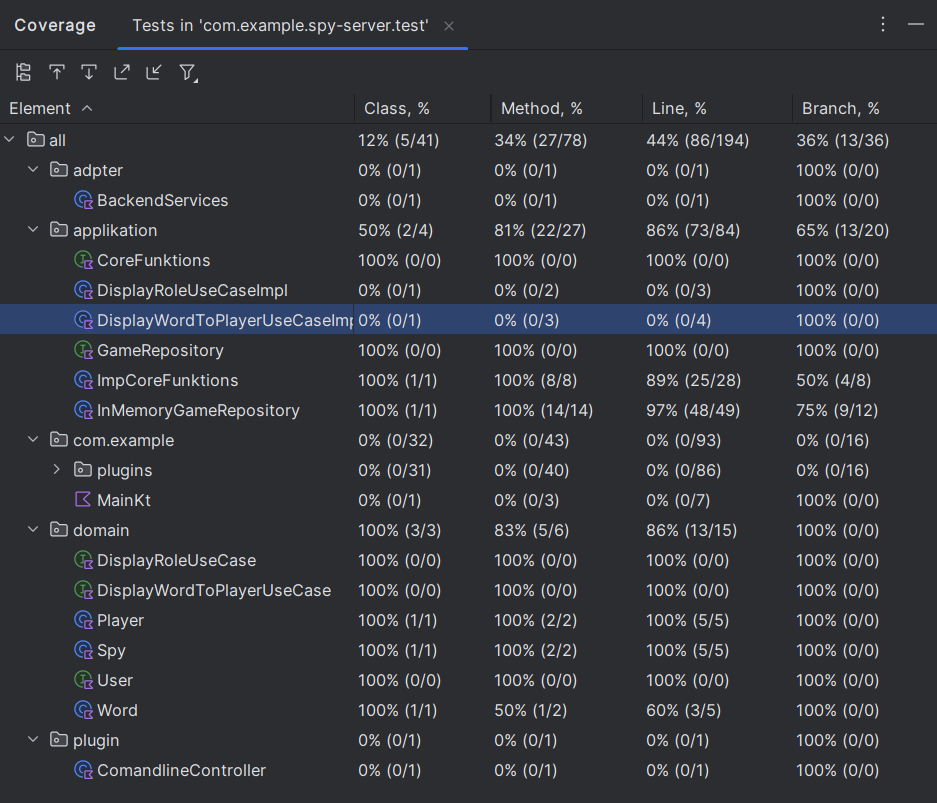
\includegraphics[width=10cm]{images/image.png}
    \caption{Code Coverage}
    \label{fig:12}
\end{figure}
Die Testabdeckung zeigt, dass derzeit nur ein kleiner Teil des Codes durch Tests abgedeckt ist.

Insgesamt beträgt die Testabdeckung für alle Klassen 12,2\%. Das bedeutet, dass nur etwa 12,2\% des Codes durch Tests getestet werden. Dies ist ein niedriger Wert und deutet darauf hin, dass viele Teile des Codes nicht ausreichend getestet wurden.

Eine detaillierte Analyse der Testabdeckung zeigt, dass einige Pakete und Klassen besser abgedeckt sind als andere:

\begin{itemize}
    \item Das Paket "applikation" hat eine Testabdeckung von 50\% für Klassen, 81,5\% für Methoden, 65\% für Verzweigungen und 86,9\% für Zeilen. Dies deutet darauf hin, dass dieses Paket besser getestet ist als andere, aber es gibt immer noch Bereiche, die verbessert werden könnten.
    
    \item Das Paket "domain" hat eine höhere Testabdeckung, mit 100\% für Klassen, 83,3\% für Methoden und 86,7\% für Verzweigungen. Dies deutet darauf hin, dass dieses Paket gründlicher getestet wurde und weniger ungetestete Bereiche aufweist.
    
    \item Die anderen Pakete wie "adpter", "com.example" und "com.example.plugins" haben eine Testabdeckung von 0\%, was darauf hindeutet, dass sie überhaupt nicht getestet wurden.
\end{itemize}

Insgesamt zeigt die Analyse der Testabdeckung, dass es noch viel Raum für Verbesserungen gibt. Eine höhere Testabdeckung ist wichtig, um die Zuverlässigkeit und Qualität des Codes sicherzustellen und potenzielle Fehler zu identifizieren. Es ist ratsam, die Testabdeckung schrittweise zu verbessern, indem mehr Tests hinzugefügt und ungetestete Bereiche abgedeckt werden.

Hier wurde die Code Coverage durch geführt \href{https://github.com/lorenz1702/Spy-Game/commit/735b2712fbacca8f45f3a4fd820081cb8efeea14}{Commit-Hash}

\newpage
\chapter{Refactoring}

\section{Code smells identifizieren}


\subsection*{Lage Class and Long Method}

\begin{lstlisting}[language=Kotlin, caption={Code Smell: Large Class and Long Method}, label={lst:5}]

class InMemoryGameRepository : GameRepository {
    
    private val users = mutableListOf<User>()
    private val players = mutableListOf<Player>()
    private val spies = mutableListOf<Spy>()
    private var words = mutableListOf<Word>()
    private var word: Word? = null

    // Add players to the repository


    fun addPlayer(player: Player) {
        players.add(player)
        users.add(player)
    }

    // Add spies to the repository
    fun addSpy(spy: Spy) {
        spies.add(spy)
        users.add(spy)
    }

    // Set the secret word
    override fun setWord(theword: Word) {
        this.word = theword
    }

    override fun getWord(): Word? {
        return this.word
    }


    // Implement methods from the GameRepository interface

    override fun createPlayer(PlayerId: Int): Player {
        return Player(
            PlayerId,
            "Player $PlayerId"
        )
    }

    override fun createSpy(SpyId: Int): Spy {
        return Spy(SpyId,"Spy $SpyId")
    }

    fun getAllWords(): MutableList<Word> {
        return this.words
    }
    override fun LoadWords() {
        val geographicZones = arrayOf(
            "Arctic",
            "Antarctic",
            "Tundra",
            "Taiga",
            "Temperate Forest",
            "Tropical Rainforest",
            "Grassland",
            "Desert",
            "Savanna",
            "Mediterranean"
        )

        words.clear() // Clear existing words
        for ((index, zone) in geographicZones.withIndex()) {
            words.add(createWord(index + 1, zone))
        }
    }

    override fun createWord(WordId: Int, Word: String): Word {

        return Word(WordId, Word)
    }

    override fun getAllUser(): List<User> {
        return users.toList()
    }



    override fun getRandomWord(): Word {
        if (words.isEmpty()) {
            throw IllegalStateException("No words available")
        }
        return words.random()
    }

    override fun createUsers(numberOfSpies: Int, numberOfPlayers: Int) {
        for (i in 1..numberOfSpies) {
            this.addSpy(createSpy(i))

        }
        for (i in 1..numberOfPlayers) {
            this.addPlayer(createPlayer(i))
        }
    }

    override fun userdisplaythereRole() {
        users.forEach { user ->
            println("${user.username}: ")
            user.displayRole()
        }
    }
}
\end{lstlisting}

Die Klasse InMemoryGameRepository zeigt mehrere Code Smells auf, die auf potenzielle Probleme im Code hinweisen. Einer dieser Code Smells ist die Größe der Klasse, die zu groß erscheint und möglicherweise mehrere Verantwortlichkeiten beinhaltet. Dies verstößt gegen das Single Responsibility Principle (SRP), das besagt, dass eine Klasse nur für eine Aufgabe verantwortlich sein sollte.

Ein weiterer Code Smell ist die Kombination von Datenverwaltung und Geschäftslogik innerhalb derselben Klasse. Die InMemoryGameRepository Klasse ist nicht nur für die Verwaltung von Daten zuständig, sondern enthält auch Logik, die sich auf das Spiel bezieht. Dies führt zu einer unklaren Trennung der Verantwortlichkeiten und kann die Wartbarkeit und Testbarkeit des Codes beeinträchtigen.

Darüber hinaus verstößt das GameRepository Interface gegen das Interface Segregation Principle (ISP). Das ISP besagt, dass Clients nicht von Methoden abhängig sein sollten, die sie nicht verwenden. Da das GameRepository Interface von der InMemoryGameRepository Klasse implementiert wird, die sowohl Datenverwaltung als auch Spiellogik enthält, kann es sein, dass Clients gezwungen sind, Methoden zu implementieren oder zu verwenden, die für sie nicht relevant sind. Dies führt zu einer Interface-Bloat und Verletzung des ISP.


\subsection*{Duplicated Code}
\begin{lstlisting}[language=Kotlin, caption={Code Smell: Duplicated Code}, label={lst:13}]
override fun loadKlimacticWords(): List<Word> {
    val words = mutableListOf<Word>()
    val geographicZones = arrayOf(
        "Arctic",
        "Antarctic",
        "Tundra",
        "Taiga",
        "Temperate Forest",
        "Tropical Rainforest",
        "Grassland",
        "Desert",
        "Savanna",
        "Mediterranean"
    )

    words.clear() // Clear existing words
    for ((index, zone) in geographicZones.withIndex()) {
        words.add(createWord(index + 1, zone))
    }
    return words
}

override fun loadSportWords(): List<Word> {
    val words = mutableListOf<Word>()
    val sportWords = arrayOf(
        "Fussball",
        "Basketball",
        "Tennis",
        "Volleyball",
        "Schwimmen",
        "Laufen",
        "Leichtathletik",
        "Boxen",
        "Handball",
        "Rugby",
        "Golf",
        "Hockey",
        "Tischtennis",
        "Badminton",
        "Radfahren",
        "Skifahren",
        "Snowboarden",
        "Klettern",
        "Tauchen",
        "Yoga"
    )
    words.clear() // Clear existing words
    for ((index, zone) in sportWords.withIndex()) {
        words.add(createWord(index + 1, zone))
    }
    return words
}
\end{lstlisting}
In diesem Code gibt es zwei ähnliche Methoden, \texttt{loadKlimacticWords} und \texttt{loadSportWords}, die beide eine Liste von Wörtern laden und zurückgeben. Beide Methoden haben folgende Gemeinsamkeiten:

\begin{enumerate}
  \item Sie erstellen eine leere Liste von Wörtern (\texttt{words.clear()}), bevor sie neue Wörter hinzufügen.
  \item Sie verwenden eine Schleife, um Wörter aus einem Array von Strings hinzuzufügen.
  \item Sie verwenden die \texttt{createWord}-Methode, um ein Word-Objekt zu erstellen und es der Liste hinzuzufügen.
\end{enumerate}

Obwohl die spezifischen Wortlisten unterschiedlich sind, ist die grundlegende Logik zum Laden der Wörter in beiden Methoden sehr ähnlich. Dies führt zu redundantem Code, da die gleichen oder ähnliche Codefragmente an mehreren Stellen im Code vorhanden sind.

Die Präsenz dieses duplizierten Codes führt zu mehreren Problemen:

\begin{itemize}
  \item Erhöhter Wartungsaufwand: Änderungen müssen an mehreren Stellen im Code vorgenommen werden, was die Wartung erschwert und die Fehleranfälligkeit erhöht.
  \item Niedrige Kohäsion: Der Code könnte kohäsiver sein, indem er die gemeinsame Logik an einem Ort konsolidiert.
  \item Wiederverwendbarkeit: Durch die Konsolidierung des Codes an einer Stelle könnte die Wiederverwendbarkeit verbessert werden, da der Code leichter in anderen Teilen des Systems verwendet werden könnte.
\end{itemize}

Daher handelt es sich hier um einen Fall von duplicated Code, der vermieden werden sollte, indem die gemeinsame Logik in eine separate Methode oder Funktion extrahiert wird, um die Wiederholung zu vermeiden.

\section{Refactoring the Code Smell}

\subsection*{Interface Segregation Principle}
\label{ISP}
Um den Code Smell Large Class zu beheben wird das Interface Segregation Principle angewendet. In dem die Datenverwaltung auszulagern und in separate Interfaces aufzuteilen: UserRepository, WordRepository und DataRepository. Jedes Interface sollte nur die Methoden enthalten, die für die Verwaltung des entsprechenden Datentyps erforderlich sind\ref{lst:6}.\\
\begin{lstlisting}[language=Kotlin, caption={Interface Segragation Principle}, label={lst:6}]
interface DataRepository {
    fun getAllUsers(): List<User>
    fun getAllWords(): List<Word>
    fun getWord(): Word?
    fun setWord(word: Word)
    fun setUser(createUsers: List<User>)
}


interface UserRepository {
    fun createSpy(spyId: Int): Spy
    fun createPlayer(playerId: Int): Player
    fun createUsers(numberOfSpies: Int, numberOfPlayers: Int): List<User>
    fun displayAllUserRoles(userList:List<User>)
}


interface WordRepository {
    fun loadWords():List<Word>
    fun createWord(wordId: Int, word: String): Word
    fun getRandomWord(words: List<Word>): Word
}
\end{lstlisting}

Zusätzlich kann die Game-Logik mit Dependency Inversion ausgelagert werden in den Domain Code. Die GameLogic-Klasse kann dann diese abstrakten Repositories verwenden, um die Daten zu verwalten und die Game-Funktionen auszuführen. Dies verbessert die Flexibilität und Testbarkeit des Codes diese wird genauer hier beschrieben \ref{sec:DI}.

Auch wurden Funktion und Code entfernt der nicht genutzt wurde\href{https://github.com/lorenz1702/Spy-Game/commit/b6fee0f44df3278afe4a151fb1b4239a373f95bf}{Commit-Hash}.


\subsection{Extract Method}

\begin{lstlisting}[language=Kotlin, caption={Extract Method}, label={lst:7}]
fun displayOneRole(){
    if (users.isEmpty()) { return }
    val randomIndex = (0..<users.size).random()
    val randomUser = users.removeAt(randomIndex)

    println("${randomUser.username}:")
    randomUser.displayRole()
    if (randomUser is Player) {
        println("Word: ${dataRepository.getWord()?.name}")  // Print the word if the user is a player and not a spy
    }
}
\end{lstlisting}

Die Methode displayOneRole \ref{lst:7} in ihrer aktuellen Form hat eine längere und komplexere Struktur, die sie schwerer zu verstehen und zu warten macht. Hier sind die Gründe, warum dies als Code Smell "Longe Method" betrachtet werden kann:

    Umfangreiche Funktionalität: Die Methode führt mehrere Aufgaben aus, darunter die Auswahl eines zufälligen Benutzers aus einer Liste, die Anzeige des Benutzernamens und seiner Rolle sowie die Anzeige des Wortes (falls der Benutzer ein Spieler ist). Diese Vielzahl von Aufgaben erhöht die Länge und Komplexität der Methode.

    Hohe Zeilenanzahl: Die Methode umfasst mehrere Zeilen Code, die verschiedene Aspekte der Logik behandeln. Dies kann dazu führen, dass Entwickler mehr Zeit benötigen, um den gesamten Code zu verstehen und potenzielle Fehler zu identifizieren.

    Schlechte Lesbarkeit: Eine lange Methode kann schwer zu lesen sein, insbesondere wenn sie viele Schritte oder bedingte Anweisungen enthält. Dies kann die Wartbarkeit des Codes beeinträchtigen und die Fehlerbehebung erschweren.

Um den Code Smell "Longe Method" zu adressieren, könnte die Methode in kleinere, spezifischere Methoden aufgeteilt werden, die jeweils eine einzelne Aufgabe ausführen. Dadurch wird der Code modularer, besser lesbar und einfacher zu warten.


Um den Code der Methode displayOneRole zu verbessern und den Code Smell "Longe Method" zu adressieren, können wir die Methode in kleinere, spezifischere Methoden aufteilen, die jeweils eine einzelne Aufgabe ausführen. Hier ist eine refrakturierte Version unter Verwendung der Methode "Extract Method":

\begin{lstlisting}[language=Kotlin, caption={Extract Method}, label={lst:7}]
fun displayOneRole() {
    if (users.isEmpty()) { return }

    val randomUser = userRepository.selctRandomUser(users)
    users.remove(randomUser)
    randomUser.displayRole()
    if (randomUser is Player) {
        printPlayerWord(randomUser)
    }
}

private fun printPlayerWord(player: Player) {
    println("Word: ${dataRepository.getWord()?.name}")
}

class ImpUserRepository : UserRepository{

override fun selctRandomUser(userList: MutableList<User>): User {
    val randomIndex = (0..<userList.size).random()
    return userList.removeAt(randomIndex)
}
}

\end{lstlisting}
In dieser refaktorierten Version wurde die ursprüngliche Methode displayOneRole in zwei kleinere Methoden aufgeteilt:

    selectRandomUser(): Diese Methode wählt einen zufälligen Benutzer aus der Liste aus und entfernt ihn dann aus der Liste.
    
    printPlayerWord(player: Player): Diese Methode druckt das Wort des übergebenen Spielers, falls vorhanden.

Durch diese Aufteilung wird der Code modularer, besser lesbar und einfacher zu warten, wodurch der Code Smell "Longe Method" behoben wird\href{https://github.com/lorenz1702/Spy-Game/commit/ef557ef3a24fecf2d3747dbc6dbf457b8c440d5c}{Commit-Hash}.

\subsection{Template Method}
In diesem Commit wird die Code duplication \ref{lst:13} mit einer Template Method und mit dem Liskov Substitutionsprinzip gelöst \ref{LSP}.

In dem refrakturierten Code ist die Verwendung des Template Method-Musters in der Klasse AbstractWordRepository deutlich erkennbar.

Das Template Method-Method definiert das Grundgerüst eines Algorithmus in einer Superklasse, ermöglicht es jedoch den Unterklassen, bestimmte Schritte des Algorithmus zu überschreiben, ohne dessen Struktur zu ändern.

In diesem Fall:
\begin{itemize}
    \item Die Klasse AbstractWordRepository definiert eine Template-Methode loadWords(), die den Algorithmus zum Laden von Wörtern repräsentiert.
    \item Die Methode loadWords() enthält gemeinsames Verhalten, das von allen Unterklassen gemeinsam genutzt wird, wie z. B. das Löschen vorhandener Wörter, das Iterieren über ein Array von Wörtern, das Erstellen von Word-Objekten und das Hinzufügen zu einer Liste.
    \item Die Methode createWord() wird innerhalb der Template-Methode verwendet, um Word-Objekte zu erstellen und bietet eine Möglichkeit für Unterklassen, den Erstellungsprozess bei Bedarf anzupassen.
    \item Unterklassen (KlimacticWordRepository und SportWordRepository) erweitern die Klasse AbstractWordRepository und überschreiben die Methode loadWords(), um spezifische Implementierungen zum Laden von klimabezogenen und sportbezogenen Wörtern bereitzustellen.
    \item Durch die Verwendung des Template Method-Musters wird der Gesamtalgorithmus zum Laden von Wörtern in der Superklasse (AbstractWordRepository) definiert, während Unterklassen bestimmte Schritte anpassen können, ohne die Gesamtstruktur des Algorithmus zu ändern.
\end{itemize}
    
Daher macht die Anwesenheit einer Methode (loadWords()) in der Superklasse, die die allgemeine Struktur des Algorithmus definiert und Haken für die Anpassung in den Unterklassen bereitstellt, das Template Method-Method deutlich erkennbar.

Den Code findet man hier unter Liskov Substitutionsprinzip\ref{LSP} oder im \href{https://github.com/lorenz1702/Spy-Game/commit/e3fef4ffb48a3b35e6825ff9a1084a08438eeed2}{Commit-Hash}.
%Zunächst muss die Klasse InMemoryGameRepository aufgeteilt werden sie hat zu viele Aufgaben sie verwaltet um einen die GameLogic, zum anderen verwaltet sie zuviele dataten die teilweise nicht verwendet werden müssen. Im Bezug auf die User, Words and the GameData das verstößt gegen das ISP.\\

%Zu nächst werden die Dataen verwaltung ausgelagert in drei interfaces UserRepository, Wordrepository and Datarepository jedes interface hat nur die Aufgabe eine Datentyp zu verwalten. Dannach habe ich die Game logik mit Dependensy Inversion ausgelagert. diese ist genauer hier beschrieben\ref{Dependancy Inversion}.

%Multibale responsibilities

%Single Responsibility Principle

%Interface Segregation Principle



%TODO: ZEITSKALEN AUF K=100 und T=10 ändern




\end{document}